\documentclass[11pt]{article}
\usepackage[margin=0.8in]{geometry}
\usepackage{lmodern,microtype,xurl,booktabs,graphicx,amsmath,amssymb,xcolor,hyperref}
\hypersetup{colorlinks=true,urlcolor=blue,linkcolor=blue,pdftitle={Release cadence improves a score but misses the review queue},pdfauthor={James N. Jean IV}}
\setlength{\parindent}{0pt}\setlength{\parskip}{6pt}
\setlength{\tabcolsep}{6pt}
\newcommand{\MSourceRows}{484}
\newcommand{\MSourceFiles}{18}
\newcommand{\MSourceBytes}{2,248,070}
\newcommand{\MNativeChecks}{6,024}
\newcommand{\MDevChecks}{8,970}
\newcommand{\MFinalChecks}{2,272}
\newcommand{\MTraining}{168}
\newcommand{\MValidation}{30}
\newcommand{\MFinal}{39}
\newcommand{\MTrainPos}{12}
\newcommand{\MValPos}{4}
\newcommand{\MFinalPos}{10}
\newcommand{\MFixtures}{21}
\newcommand{\MDeps}{32}
\newcommand{\MCandidates}{9}
\newcommand{\MShortN}{154}
\newcommand{\MShortPos}{7}
\newcommand{\MLongN}{14}
\newcommand{\MLongPos}{5}
\newcommand{\MTP}{0}
\newcommand{\MFP}{0}
\newcommand{\MFN}{10}
\newcommand{\MTN}{29}
\newcommand{\MBaseDev}{0.323495}
\newcommand{\MSelectedDev}{0.233250}
\newcommand{\MBaseFinal}{0.286162}
\newcommand{\MSelectedFinal}{0.249727}
\newcommand{\MBaseMicro}{0.223042}
\newcommand{\MSelectedMicro}{0.191728}
\newcommand{\MBaseLog}{0.903990}
\newcommand{\MSelectedLog}{0.809713}
\newcommand{\MBaseP}{0.076471}
\newcommand{\MShortP}{0.045655}
\newcommand{\MLongP}{0.338431}
\newcommand{\MHTTPXBaseLog}{1.574331}
\newcommand{\MHTTPXSelectedLog}{1.616603}
\newcommand{\MRepoASource}{27}
\newcommand{\MRepoATraining}{9}
\newcommand{\MRepoAValidation}{1}
\newcommand{\MRepoAFinal}{0}
\newcommand{\MRepoBSource}{51}
\newcommand{\MRepoBTraining}{0}
\newcommand{\MRepoBValidation}{0}
\newcommand{\MRepoBFinal}{5}
\newcommand{\MRepoCSource}{30}
\newcommand{\MRepoCTraining}{9}
\newcommand{\MRepoCValidation}{4}
\newcommand{\MRepoCFinal}{0}
\newcommand{\MRepoDSource}{57}
\newcommand{\MRepoDTraining}{0}
\newcommand{\MRepoDValidation}{0}
\newcommand{\MRepoDFinal}{11}
\newcommand{\MRepoESource}{38}
\newcommand{\MRepoETraining}{12}
\newcommand{\MRepoEValidation}{8}
\newcommand{\MRepoEFinal}{0}
\newcommand{\MRepoFSource}{19}
\newcommand{\MRepoFTraining}{0}
\newcommand{\MRepoFValidation}{0}
\newcommand{\MRepoFFinal}{6}
\newcommand{\MRepoGSource}{177}
\newcommand{\MRepoGTraining}{138}
\newcommand{\MRepoGValidation}{17}
\newcommand{\MRepoGFinal}{0}
\newcommand{\MRepoHSource}{85}
\newcommand{\MRepoHTraining}{0}
\newcommand{\MRepoHValidation}{0}
\newcommand{\MRepoHFinal}{17}
\begin{document}
\begin{center}
{\LARGE\bfseries Release cadence improves a score\\but misses the review queue}\par
\vspace{8pt}James N. Jean IV\\
Independent research and implementation study\quad 30 October 2026\\
{\small Reproducible candidate, not peer reviewed}
\end{center}
\section*{Decision brief}
A dependency owner may need time to inspect a project's release process before an upgrade deadline. This study tests whether three past stable-release intervals help identify a subsequent ninety-day gap in stable GitHub releases. The outcome is a recorded publishing pattern; actual maintenance activity is unobserved.

The frozen cadence rule improves final macro Brier score from \MBaseFinal{} to \MSelectedFinal{} on \MFinal{} origins from four other projects. Its predeclared probability-at-least-one-half review rule flags none of the \MFinalPos{} observed gaps. The probabilistic comparison improves, while the review output fails to surface any positive case.

\begin{center}\begin{tabular}{lrr}\toprule
Final outcome & Pooled baseline & Frozen cadence rule\\\midrule
Macro Brier, lower is better & \MBaseFinal & \MSelectedFinal\\
Micro Brier, lower is better & \MBaseMicro & \MSelectedMicro\\
Macro log loss, nats & \MBaseLog & \MSelectedLog\\
Observed gaps flagged & 0/\MFinalPos & \MTP/\MFinalPos\\
Observed gaps missed & \MFinalPos & \MFN\\\bottomrule
\end{tabular}\end{center}

\textbf{Practical recommendation.} Keep cadence as contextual evidence in a dependency review, with the release channel and actual maintenance evidence attached. The tested threshold produces an empty queue and should not serve as an automatic routing policy. A prospective evaluation should measure the decisions and outcomes a dependency owner actually cares about.

\textbf{Evidence boundary.} Eight familiar Python-tooling repositories form an authored cohort in a current public snapshot. Edited or deleted releases prevent an original-vintage reconstruction. Origins overlap, and projects share organizations and an ecosystem. There is no representative sample or independent maintenance-status label. Deployment benefit, abandonment and security outcomes are unmeasured.

\textbf{Usable output.} Saved minimal metadata, a fixed model, all candidates, independent checks and an offline exercise support a contextual review item without contacting a maintainer.
\newpage
\section*{1. What the source actually measures}
GitHub's releases endpoint lists published release records; ordinary Git tags without a release use a separate endpoint. Stable here means captured draft and prerelease flags are both false. Projects can publish packages or continue development through other channels. The target concerns stable GitHub release cadence only.

The snapshot contains \MSourceRows{} release entries from \MSourceFiles{} preserved response entities totaling \MSourceBytes{} decoded bytes: one initial public rate-limit response, eight repository metadata responses and nine release-list pages. Acquisition follows publisher pagination to its actual end. All repositories are public non-forks in current metadata.

\begin{center}\small\begin{tabular}{llrrrr}\toprule
Repository & Group & Source & Train & Valid. & Final\\\midrule
python-attrs/attrs & Development & \MRepoASource & \MRepoATraining & \MRepoAValidation & \MRepoAFinal \\
encode/httpx & Final & \MRepoBSource & \MRepoBTraining & \MRepoBValidation & \MRepoBFinal \\
pallets/click & Development & \MRepoCSource & \MRepoCTraining & \MRepoCValidation & \MRepoCFinal \\
psf/black & Final & \MRepoDSource & \MRepoDTraining & \MRepoDValidation & \MRepoDFinal \\
pallets/flask & Development & \MRepoESource & \MRepoETraining & \MRepoEValidation & \MRepoEFinal \\
psf/requests & Final & \MRepoFSource & \MRepoFTraining & \MRepoFValidation & \MRepoFFinal \\
Textualize/rich & Development & \MRepoGSource & \MRepoGTraining & \MRepoGValidation & \MRepoGFinal \\
pytest-dev/pytest & Final & \MRepoHSource & \MRepoHTraining & \MRepoHValidation & \MRepoHFinal \\
\bottomrule\end{tabular}\end{center}

The assignment sorts SHA256 values of lowercase repository slugs and alternates development and final groups before acquisition. Distinct IDs do not establish independent projects. Source counts include excluded entries and dates outside the origin windows. Every qualification reason is retained.

Complete responses remain private. Public files contain IDs, timestamps, state flags, hashes and new calculations, excluding release prose, profiles, avatars and assets. Local hashes describe Requests-decoded entities rather than publisher checksums. The original GH Archive proposal was narrowed before acquisition because its software/documentation license does not blanket-license archived third-party event content. Contributor concentration and bot attribution are not executed analyses.

The first collector stopped at a numeric repository-ID next link rejected by its initial named-path guard. Fifteen successful originals and the code are preserved. A correction accepts the exact verified ID while retaining origin/page restrictions. One continuation reused all prior bodies after hash checks and made three new requests. Six pagination fixture methods cover the correction. No denied source or outcome-dependent cohort change was involved.
\newpage
\section*{2. A fixed model with a retained search}
At each eligible origin, the predictor is the median of the three most recent elapsed release intervals, including the interval ending at that origin. Events sort by publication time then release ID; a same-time later release ends the next interval at zero. Missing timestamps, insufficient history and incomplete windows retain separate exclusion reasons.

Training uses development-project origins in 2020--2022 with ninety-day windows ending by the training boundary. Validation uses those projects' 2023 origins with windows ending by its boundary. The target is $y=1$ when no next stable release occurs within ninety elapsed days; an event exactly at the horizon counts as within it. Training has \MTraining{} origins and \MTrainPos{} gaps; validation has \MValidation{} origins and \MValPos{} gaps.

For training count $n$ and positives $k$, the authored pooled baseline is $p_0=(k+1)/(n+2)$. Candidate cutpoints are 14, 30 and 60 days; prior strengths are 1, 5 and 20. Each stratum uses
\[
 p_s=\frac{k_s+a p_0}{n_s+a}.
\]
Empty strata return $p_0$. All \MCandidates{} authored hypotheses and runtimes are retained. They imply no global-optimum claim.

\begin{center}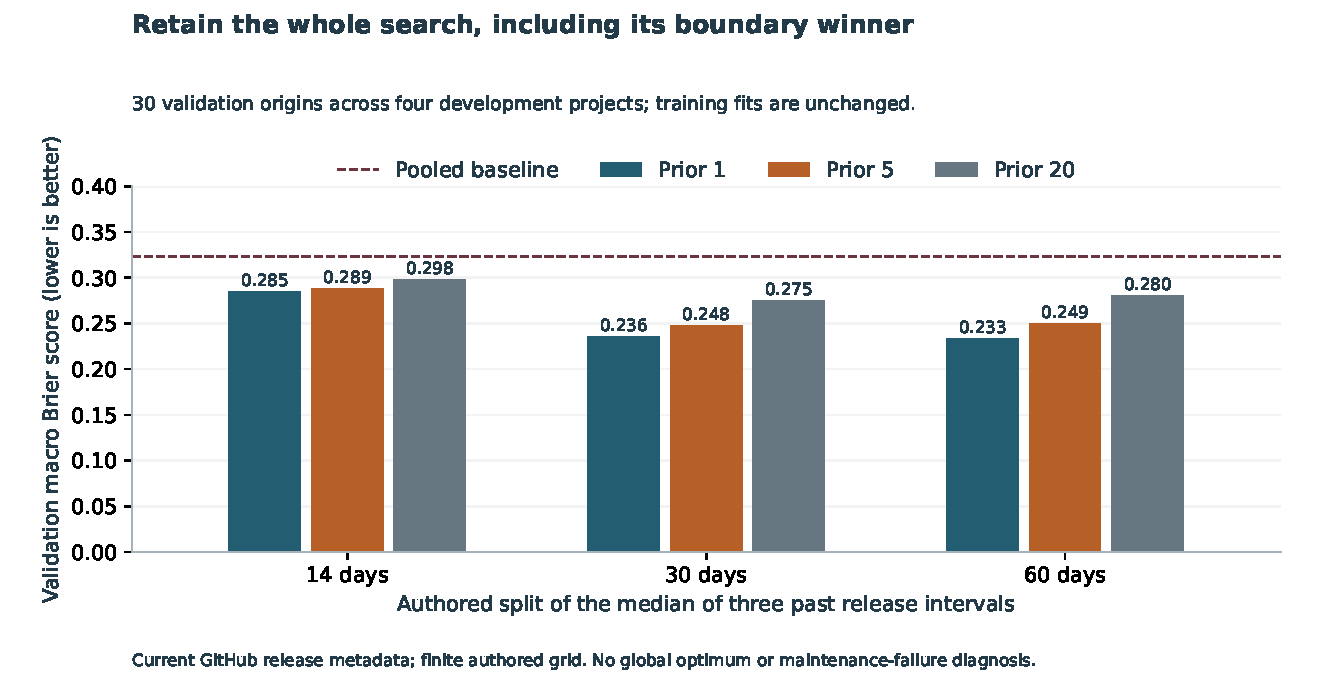
\includegraphics[width=\linewidth]{images/validation_search.pdf}\end{center}
Selection minimizes validation Brier averaged equally across projects; exact ties favor a larger prior then smaller cutpoint. The selected 60-day split and prior 1 are boundary winners. Validation macro Brier is \MSelectedDev{} versus \MBaseDev{}. There is no validation refit. A committed manifest of \MDeps{} dependencies precedes final feature, label and score extraction. Source envelopes already contain final metadata, so collection was not blinded.
\newpage
\section*{3. Other projects and later origins}
Final evaluation applies the unchanged training fit to the other four projects' 2024--2025 origins, with full windows ending by the final boundary. There are \MFinal{} origins and \MFinalPos{} gaps. No final outcome chooses a new cutpoint, prior, horizon or threshold.

\begin{center}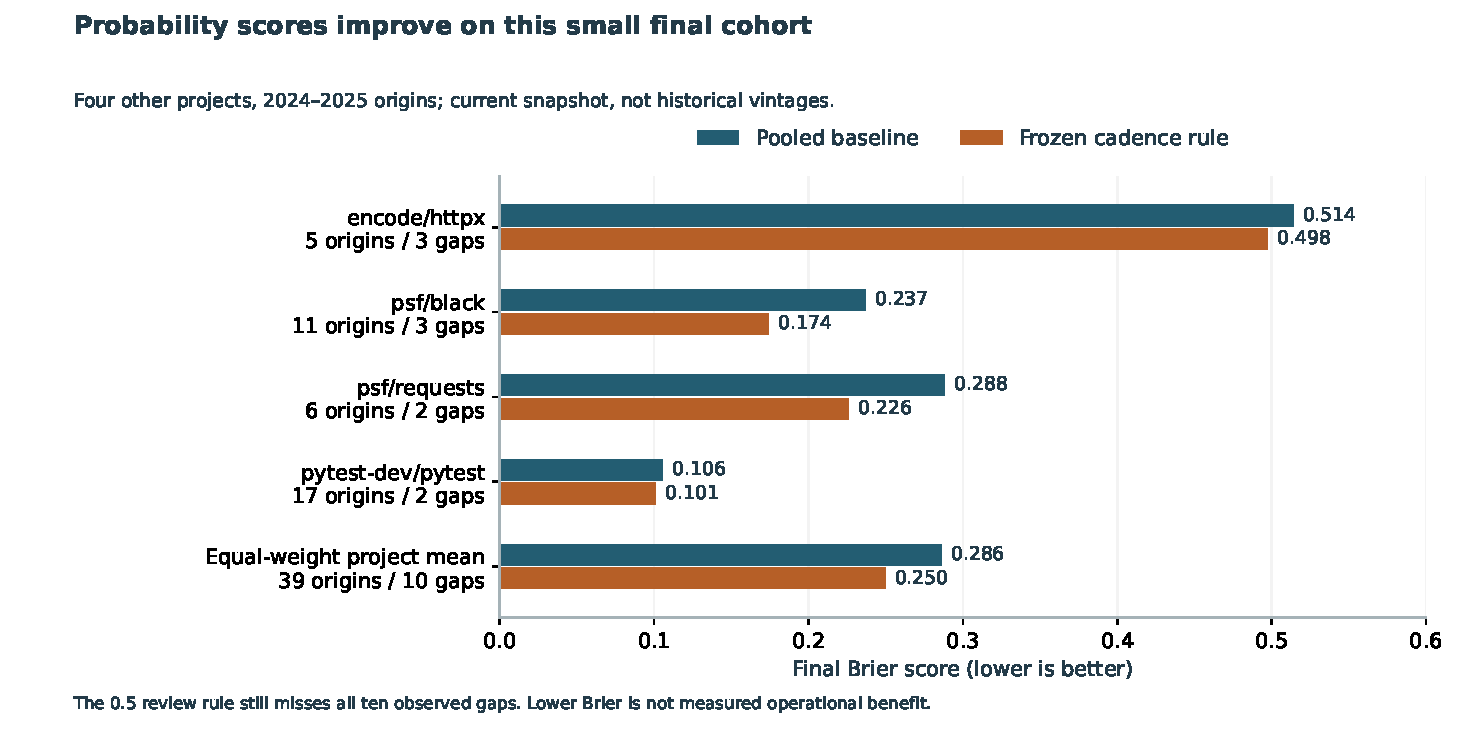
\includegraphics[width=\linewidth]{images/project_scores.pdf}\end{center}

Macro Brier weights projects equally; micro Brier weights origins equally. Both improve on this finite cohort. Each project's Brier is lower for the cadence rule. Other scores can worsen: encode/httpx log loss rises from \MHTTPXBaseLog{} to \MHTTPXSelectedLog{} nats in a subgroup with five origins and three gaps.

The training baseline probability is \MBaseP{}. The selected shorter-cadence stratum has \MShortN{} training origins and \MShortPos{} gaps, while its longer-cadence stratum has \MLongN{} origins and \MLongPos{} gaps. The resulting probabilities are \MShortP{} and \MLongP{}. Both remain below the authored review threshold.

Separate IDs and later dates preserve the declared split while leaving ecosystem dependence and current snapshot omissions unresolved. A difference in cadence does not identify a causal effect of contributor behavior or dependency policy. Actual outages, avoided costs, workload reductions and security outcomes are outside the observed data.
\newpage
\section*{4. The review failure is part of the result}
At $p\geq0.5$, final counts are true positives \MTP{}, false positives \MFP{}, false negatives \MFN{} and true negatives \MTN{}. Precision is undefined because no flags are emitted. Recall is zero of \MFinalPos{} observed gaps. The baseline also emits no flags. The threshold remains unchanged after final inspection.

\begin{center}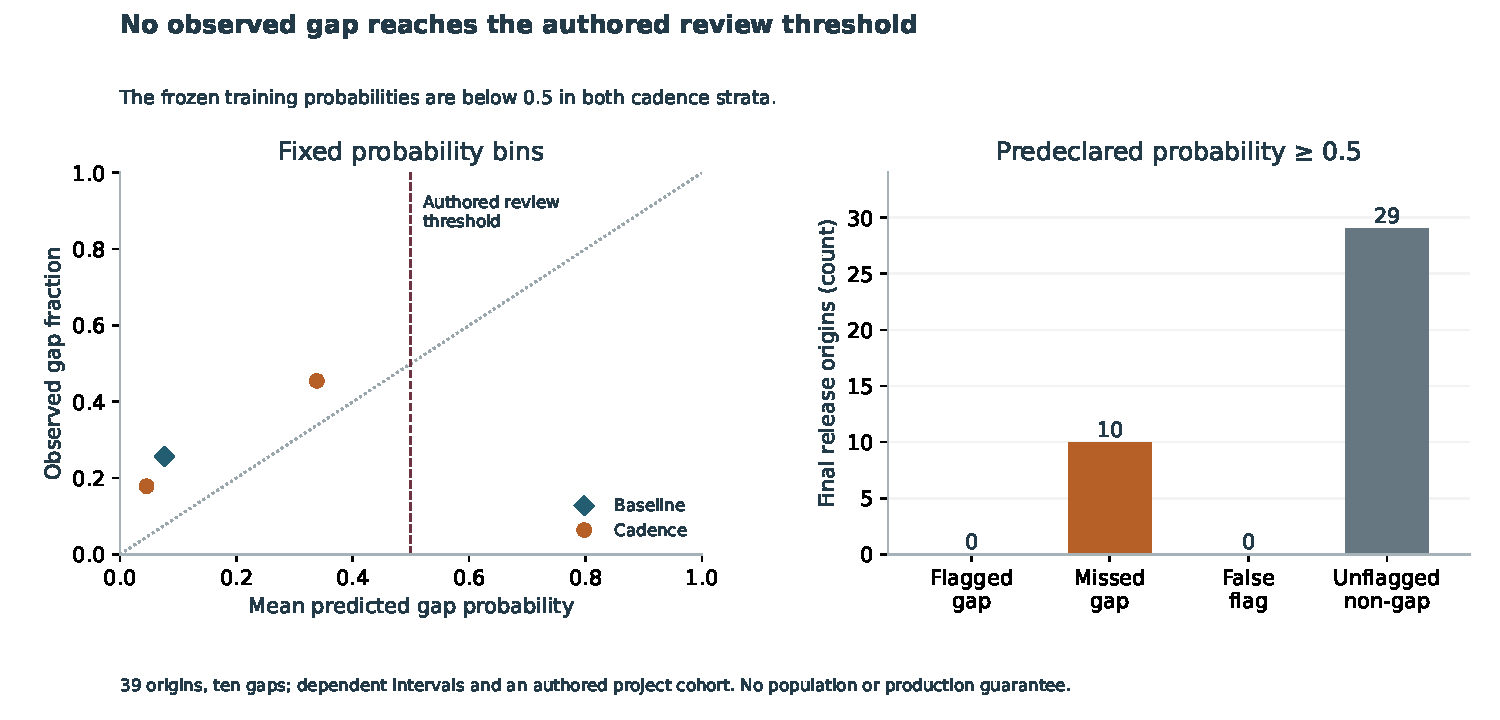
\includegraphics[width=\linewidth]{images/calibration_and_misses.pdf}\end{center}

Fixed probability bins show underprediction. The selected shorter-cadence bin contains 28 origins with five gaps; the longer-cadence bin contains eleven origins with five gaps. Both frequencies exceed their frozen probabilities. Lower aggregate Brier is not a calibration certificate; Brier and log loss reflect more than calibration alone.

Separate descriptive product-limit summaries use observed inter-release durations and right-censoring at each phase boundary. At ninety days, full-window inclusion makes the final empirical remaining-gap fraction ten of thirty-nine. Overlapping origins and current source omissions prevent an independent-sampling interpretation or project-level survival diagnosis.

The offline exercise accepts three authored integer day intervals and returns an estimate with its scope. It makes no requests, sends no notification and replaces no dependency. A useful next study would prospectively record release channels, review decisions and actual maintenance outcomes across a broader cohort before selecting an operational policy.
\newpage
\section*{5. Reproducibility and checks}
DuckDB JSON and SQL reconcile exact private response entities to minimal public source fields in \MNativeChecks{} conditions. A separate SQLite window implementation rebuilds chronology. Fraction arithmetic checks probabilities, Brier and denominators; 75-digit Decimal log-loss comparisons use tolerance $2\times10^{-12}$. Development checks cover \MDevChecks{} conditions, final checks \MFinalChecks{}. These finite checks do not establish universal reliability.

\MFixtures{} fixture methods cover chronology, horizon boundaries, same-time ordering, missing/timezone data, source flags, empty strata, undefined denominators, log flooring, selection ties, risk sets and pagination identity. Initial measured runtimes are retained; replay writes fresh runtime receipts separately. Current-checkout development replays ran under CPython 3.10.11 and 3.12.14.

\begin{verbatim}
python -m unittest discover -s tests -v
python src/freeze_proof.py
python src/replay.py --output ../fresh-replay
python src/review_cli.py examples/authored-intervals.json
python src/verify_figures.py
\end{verbatim}
Use a fresh output outside the checkout. Captured-source replay makes no new network requests. Runtime is provenance rather than expected replay bytes. Public replay checks saved minimal facts and source proof; private originals remain excluded. Release requires an isolated full-history replay, source/figure hashes, actual SVG geometry, every rendered paper page, a scoped publication audit and exact GitHub CI/tree/tag evidence. Check the chosen revision's evidence when using this package.

\section*{Primary sources and method references}
\small
GitHub. \emph{REST API endpoints for releases}; pagination and rate-limit documentation. \url{https://docs.github.com/en/rest/releases/releases}. Published release records differ from ordinary Git tags.

GH Archive. \emph{Licenses}. \url{https://github.com/igrigorik/gharchive.org#licenses}. Software and website rights differ from third-party event rights.

NIST/SEMATECH. \emph{Empirical model fitting: Kaplan--Meier approach}. \url{https://www.itl.nist.gov/div898/handbook/apr/section2/apr215.htm}. Product-limit summaries here are descriptive.

scikit-learn developers. \emph{Probability calibration}. \url{https://scikit-learn.org/stable/modules/calibration.html}. Brier and log loss assess more than calibration alone. The small model is implemented directly, without a scikit-learn dependency.

\normalsize\textbf{Publication scope.} This independent manuscript is eligible for the reviewed program subset. Separate formal-publication projects, including Azure optimization, remain private. Third-party prose, profiles and manuscripts are excluded.
\end{document}
